% Science submission typography; scientific text retained apart from declared format edits.
% Source: wind342/gfg-training-learning-inference-experiments
% Commit: effbe99b0b8299bc1e457a309339dc85d722c1f8
\documentclass[12pt,letterpaper]{article}
\pdfminorversion=7
\usepackage[T1]{fontenc}
\usepackage[utf8]{inputenc}
\usepackage{amsmath,amssymb}
\usepackage{mathptmx}
\usepackage[letterpaper,margin=1in]{geometry}
\usepackage{graphicx,array,booktabs}
\usepackage{microtype}
\usepackage[numbers,sort&compress,round]{natbib}
\usepackage[font=normalsize,labelfont=bf,labelsep=period]{caption}
\usepackage[hidelinks]{hyperref}
\urlstyle{same}
\linespread{1.5}
\frenchspacing
\setlength{\emergencystretch}{1em}
\setcounter{topnumber}{4}
\setcounter{bottomnumber}{4}
\setcounter{totalnumber}{6}
\renewcommand{\topfraction}{.95}
\renewcommand{\bottomfraction}{.90}
\renewcommand{\textfraction}{.05}
\renewcommand{\floatpagefraction}{.50}
\setlength{\floatsep}{12pt plus 2pt minus 2pt}
\date{}
\setcounter{secnumdepth}{0}
\captionsetup[figure]{name=Fig.}
\makeatletter
\renewcommand{\maketitle}{\begin{center}\vspace*{-1em}{\Large\bfseries\@title\par}\vspace{1em}{\normalsize\@author\par}\end{center}\vspace{.5em}}
\makeatother
% Keep original heading words and reference numbering under the verbatim constraint.
\renewcommand{\citenumfont}[1]{\textit{#1}}
\renewcommand{\bibnumfmt}[1]{#1.}
\setlength{\bibsep}{6pt}
\renewcommand\refname{References and Notes}
\renewenvironment{abstract}{\begin{quotation}\bfseries}{\end{quotation}}
\newcommand{\dd}{\Delta\theta_t}
\newcommand{\id}{\mathrm{id}}
\newcommand{\PASS}{\textsc{Pass}}
\title{\bfseries Unified Training--Learning--Inference--Reinforcement Dynamics Across Neural Systems}
% Author details supplied by the user; official English affiliation verified.
\author{wangmian\\
{\small Wuhan Polytechnic University, Wuhan, China}\\
{\small Corresponding author. Email: \href{mailto:wangmian945@gmail.com}{wangmian945@gmail.com}}}
\hypersetup{pdftitle={Unified Training--Learning--Inference--Reinforcement Dynamics Across Neural Systems},pdfauthor={wangmian}}
\begin{document}
\maketitle
\begin{abstract}
Although training, learning, inference, and reinforcement have been extensively studied, their distinct dynamical roles and connections have lacked a unified experimental characterization. Nine nanoGPT experiments established training--learning--inference relations: realized updates elicit state-dependent finite-amplitude responses, learning reorganizes distributed functional support across capability boundaries, and inference recruits that support without changing the learned state. Factors identified in the fifth experiment yielded a direct predictor of post-update capability transitions, achieving 91.43\% accuracy and 91.49\% four-way macro recall across 5,088 targets. We tested these relations and prediction across five additional neural architectures. In a seventh system, concentrated correct feedback eroded previously mastered skills; rebalanced feedback restored their accuracy from 70.31\% to 99.48\%. Linking inference consequences to subsequent training closes these relations into unified training--learning--inference--reinforcement dynamics.
\end{abstract}

\noindent
Training, generalization, capability formation, and inference are central problems in neural-network research. Different fields have developed influential theories to study them.

In \emph{optimization theory}, the Neural Tangent Kernel (NTK) describes parameter-induced output changes through the network Jacobian and the corresponding kernel in specified training regimes \cite{jacot2018}. Edge of Stability studies training behavior in relation to the largest Hessian eigenvalue, learning rate, and loss trajectory \cite{cohen2021}. Sharpness-Aware Minimization (SAM) constructs training updates using loss changes in a parameter neighborhood to improve generalization \cite{foret2021}. Here, the \emph{current state} is represented by parameters and their local derivatives or curvature; \emph{realized updates} are produced by the optimizer; and \emph{responses} appear as changes in model outputs or loss.

In \emph{representation learning and generalization}, Spectral Bias examines frequency-dependent learning rates of functions or kernel modes \cite{rahaman2019}. Implicit Bias studies why an optimizer selects particular solutions, such as maximum-margin directions on separable data \cite{soudry2018}. Neural Collapse measures class-feature means, within-class variability, and classifier geometry, revealing continuing representational change after training accuracy saturates \cite{papyan2020}. Information Bottleneck theory studies mutual information among inputs, hidden representations, and targets, including the retention and compression of task-relevant information \cite{tishby2015}. Their \emph{internal organizations} take the form of spectral modes, optimizer-selected solutions, feature geometry, or information structure; their \emph{functional changes} appear in learning rates, evolving solutions, and predictive performance.

In \emph{capability formation}, Grokking captures the long delay between fitting training examples and achieving strong test generalization \cite{power2022}. Subsequent circuit studies track the formation and reorganization of internal computations during this delay \cite{nanda2023}. Double Descent studies how test error can rise near interpolation and fall again as model size, training time, or data conditions change \cite{belkin2019,nakkiran2020}. These studies measure the \emph{current state} through training phase or interpolation regime, \emph{internal change} through circuit and solution evolution, and \emph{observable capability} through accuracy and generalization error.

In \emph{continual learning}, catastrophic forgetting occurs when training on a new task reduces performance on earlier tasks. Elastic Weight Consolidation (EWC) estimates parameter importance using Fisher information from earlier tasks and penalizes changes to important parameters \cite{kirkpatrick2017}. Gradient Episodic Memory (GEM) constrains new-task gradients using their inner products with previous-task gradients \cite{lopezpaz2017}. Orthogonal Gradient Descent (OGD) projects new gradients into directions that approximately preserve earlier-task outputs \cite{farajtabar2020}. In these methods, the \emph{existing state} includes previously learned parameters and function-sensitive directions; \emph{updates} are constrained new-task actions; \emph{interactions} occur through overlapping gradient or functional subspaces; and \emph{capability changes} are measured as retention, forgetting, or transfer.

In \emph{inference research}, Attention uses queries, keys, and values to compute input-dependent information weights \cite{vaswani2017}. In-context learning studies how examples and task information provided in the context affect predictions while model parameters remain fixed \cite{brown2020}. Chain-of-Thought prompting studies how intermediate reasoning steps affect performance on complex tasks \cite{wei2022}. The \emph{current state} is the trained model; \emph{input conditions} include the query, context, and intermediate computations; \emph{internal computation} varies with attention and activations; and \emph{functional performance} is observed in the resulting predictions.

In \emph{reinforcement and feedback-driven training}, reinforcement learning from human feedback (RLHF) uses preference and reward signals to adjust model behavior \cite{ouyang2022}. Self-training creates further training data from a model's predictions \cite{xie2020}. Recursive model-collapse studies examine the loss of low-probability modes when successive models are trained on data generated by their predecessors \cite{shumailov2024}. Here, \emph{feedback} is supplied through rewards, preferences, or generated-data distributions; \emph{training actions} are the resulting updates; and subsequent \emph{functional change} is observed through behavior, accuracy, and generated distributions.

These studies use different mathematical objects---kernels, Hessians, gradients, class features, mutual information, task scores, attention weights, and reward signals---yet six recurring categories can be identified: \emph{current state, realized update, functional response, internal organization, observable capability, and feedback}. \emph{The core TLI relations were established experimentally before this cross-field comparison; identifying these recurring variables here is a way to help readers understand the theory, not the process by which it was discovered.}

Figure~\ref{fig:chain} illustrates the four linked dynamical roles.





\section{Experimental Establishment of TLI Open-Loop Dynamics}
The nine nanoGPT experiments that established TLI involved a substantially broader set of native interventions, controlled comparisons, and independent validations than can be presented within the main text. This section summarizes their key experimental findings and the resulting theoretical relations. Complete protocols, execution records, negative results, and independent validators are provided in the accompanying repository.

\subsection{Experimental Instruments and Evidence Control}
These experiments required four instruments invented and developed by AI scientific agents, including OpenAI Codex and ChatGPT, as the measurement questions arose rather than being assumed before the theory. Under the author's scientific direction, the AI systems also designed, implemented, and executed the experiments. Their common evidence substrate was the Generation-Fact Graph (GFG), which links recorded model and optimizer states, actual update occurrences, interventions, outputs, and their source identities. For Training, realized-update causal forks restored matched receiving states and compared full, skipped, parameter-only, optimizer-memory, and reciprocal transfers, separating an update from the state on which it acts. A finite-amplitude path instrument then applied the same recorded update at frozen amplitude values to measure nonlinear numerical responses and discrete transitions. For Learning, CSRG-4C used repeated baseline, single-component, and paired-component gates to measure necessity, backup, substitution, synergy, and failure slack in the functional support of individual targets. Finally, an identity-aligned boundary ledger joined each registered target to the exact pre-update state and realized update, then separated pre-response records from post-update adjudication of correctness. The instruments enabled the subsequent experimental tests; frozen protocols, negative controls, and independent validators constrained their interpretation.

\subsection{Training: Realized Updates and Receiving States}
At a registered training step, the parameter--optimizer state is $Z_t=(\theta_t,\omega_t)$, and the realized parameter update is $\Delta\theta_t=\theta_{t+1}-\theta_t$.

TL-E01 revealed capability formation, decline, and recovery that could not be fully characterized by loss, accuracy, or training step alone. TL-E02 further showed that pausing effective parameter--optimizer evolution delays capability formation, while the clipping-threshold control did not reproduce this effect.

TL-E03 used full/skip branches and reciprocal update transplants to establish that the same realized update produces different functional responses in different receiving states:
\begin{equation}
 R_q(\theta_A,\Delta\theta_B)\quad\text{vs.}\quad R_q(\theta_B,\Delta\theta_B),
 \label{eq:receiver}
\end{equation}
where $R_q(\theta,\Delta)=m_q(\theta+\Delta)-m_q(\theta)$. Separate optimizer-memory exchanges examined how historical optimizer states affect update formation:
\begin{equation}
 \Delta^{(a,b)}=\operatorname{OptStep}(\theta_t,g_t,\omega_{a,b}).
 \label{eq:optmem}
\end{equation}
TL-E04 measured the complete finite-amplitude response to an actual update:
\begin{equation}
 r_{t,q}(\alpha)=m_q(\theta_t+\alpha\Delta\theta_t)-m_q(\theta_t).
 \label{eq:response}
\end{equation}
The experiments identified near-linear, saturating, accelerating, turnback, and sign-reversal responses. TL-E05 subsequently identified three primary response-conditioning families: target-boundary state (F1), target-specific update geometry (F3), and parameter--optimizer receiving state (F5).

\subsection{Learning: Distributed Support and Capability Boundaries}
TL-E06 used reversible component interventions to establish distributed functional support, including component necessity, backup, substitution, synergy, and failure slack.

TL-E07 then examined how realized training updates persistently reorganize this support:
\begin{equation}
 \Delta P_{t,q}=P_q(\theta_t+\Delta\theta_t)-P_q(\theta_t).
 \label{eq:realloc}
\end{equation}
Across 72 experimental sections, 1,636 valid support-allocation transitions and 228 primary-support hand-offs were recorded.

TL-E08 linked these internal changes to observable capability through identity-aligned target readout boundaries. The signs of the pre- and post-update margins distinguish maintenance, loss, non-acquisition, and acquisition or recovery. Learning is thus identified with persistent functional reorganization, while capability transitions are determined by crossings of target-specific readout boundaries.

\subsection{Inference: Frozen Recruitment of Learned Support}
INF-E01 examined 13 nanoGPT training histories and 52 checkpoints. With persistent learned states frozen, the experiment measured query-conditioned component effects, non-additive support interactions, and changes produced by replacing trained components with their exact pre-formation versions.

At a fixed learned state $L^*$, inference recruits and combines learned support:
\begin{equation}
 S_{q,c}^{\mathrm{active}}=\Pi_{q,c}(L^*),\qquad
 y_{q,c}=H_{q,c}(S_{q,c}^{\mathrm{active}}).
 \label{eq:inference}
\end{equation}
Non-additive component interactions are measured by
\begin{equation}
 I_{ij,q}=f_{\mathrm{full}}-f_{-i}-f_{-j}+f_{-i,-j},
 \label{eq:interaction}
\end{equation}
while learned-version dependence is tested through
\begin{equation}
 D_{j,q}=f(q;\theta^*)-f(q;\theta^{(j\leftarrow\mathrm{pre})}).
 \label{eq:rollback}
\end{equation}
Exact restoration verified that these interventions did not persistently alter the learned state. The experiments establish Inference as the query-conditioned recruitment and combination of support formed through Learning.

Together, these nine experiments established the connected Training--Learning--Inference relations, forming the TLI open-loop dynamics. Figure~\ref{fig:tlir-evidence} summarizes the experimental evidence across all four TLIR roles.




\section{Prediction and Cross-System Validation}
\subsection{Theory-Derived Target-Boundary Prediction}
The response-factor analysis in TL-E05 identified three primary conditioning factors: the current target-boundary state (F1), target-specific update geometry (F3), and parameter--optimizer receiving state (F5). These findings led directly to TL-P01, a predictor of immediate target-boundary outcomes following an actual formed update.

For target $y$, competitor $c$, and hidden representation $h$, let $b_c=w_y-w_c$ and $\Delta b_c=\Delta w_y-\Delta w_c$. Using the first and second directional derivatives $h'=Dh[\Delta\theta_t]$ and $h''=D^2h[\Delta\theta_t,\Delta\theta_t]$, the predictor computes
\begin{equation}
 \begin{aligned}
 \widehat g_{y,c}={}&b_c^\top h+\Delta b_c^\top h+b_c^\top h'\\
 &+\Delta b_c^\top h'+\tfrac12 b_c^\top h''.
 \end{aligned}
 \label{eq:predict}
\end{equation}
The target is predicted correct if $\min_{c\ne y}\widehat g_{y,c}>0$. Combining predicted post-update correctness with the known pre-update state gives four capability transitions. Predictions use the already formed update and pre-response information, without reading actual post-update target outputs.

\subsection{Cross-System Validation}
We subsequently tested the established TLI relations and their predictive consequences in five additional neural systems. Table~\ref{tab:systems} summarizes the seven systems used in the study, including the separate GRU reinforcement experiment examined in the reinforcement section.



Each of the five additional TLI systems was examined through realized-update interventions, receiving-state comparisons, finite-amplitude responses, component-coalition support measurements, target-boundary outcomes, and frozen-inference tests. Cross-system implementations evaluated all 16 coalitions of four registered components, with exact Shapley effects:
\begin{equation}
 \phi_{j,q}=\!\!\sum_{C\subseteq\mathcal C\setminus\{j\}}
 \frac{|C|!(3-|C|)!}{4!}\left[v_q(C\cup\{j\})-v_q(C)\right].
 \label{eq:shapley}
\end{equation}
Here $v_q(C)$ denotes the target margin under active component coalition $C$.

All 42 ResNet, 18 diffusion U-Net, and 36 Vision-MoE parameter receiving-state exchanges exceeded their registered response-difference thresholds. Finite-amplitude nonlinear responses occurred in 32.23\%, 19.25\%, and 35.71\% of their respective target-update records, while support reallocation exceeded its specified threshold in 91.41\%, 97.02\%, and 80.43\%. Their frozen-inference experiments further confirmed query-conditioned support, non-additive interactions, and dependence on exact trained component versions.

The GNN reproduced the main TLI relations across three seeds, although one seed failed the registered nonlinear-response frequency criterion (1.56\%). The hard-spiking SNN passed all twelve registered TLI criteria across four seeds, extending the evidence to discontinuous spiking dynamics.



The prediction algorithm was also evaluated across these systems, with task-specific adaptations of the directional response computation. Table~\ref{tab:prediction} reports immediate post-update target-boundary classification.



The predictor achieved high four-way recall in five systems. In the hard-spiking SNN, discontinuous activation thresholds limited local derivative-based prediction, yielding 70.74\% macro recall despite 95.31\% accuracy. Together, the experiments demonstrate cross-system recurrence of the core TLI relations and identify architecture-dependent differences in their quantitative responses and predictive approximations. Figure~\ref{fig:systems} summarizes the six within-system TLI experiment chains.

\section{Reinforcement: From TLI Open-Loop to TLIR Closed-Loop Dynamics}
\label{sec:reinforcement}
\subsection{Theory-Derived Prediction of Feedback Dynamics}
The established TLI relations show that training persistently reorganizes distributed functional support, while inference recruits and combines this learned support to produce behavior. When the consequences of inference are repeatedly fed back into subsequent training, the resulting updates can further reorganize the support on which future inference depends.

This led to a prediction: sustained, narrowly concentrated correct positive feedback could progressively favor the reinforced capability while weakening other already mastered capabilities. The predicted effect arises from feedback-directed functional reorganization, rather than incorrect rewards.

\subsection{Experimental Tests and Results}
RL-E05/E06 tested this prediction in a seventh system, a shared attention-free GRU policy. All four skills reached mastery before the experimental branches began. Every branch started from an identical parameter--AdamW state, and each complete two-decision episode received $r=1$ only when correct, and $r=0$ otherwise.

RL-E05 compared selective, balanced, and frozen feedback. RL-E06 further varied the allocation of 60 episodes per update over 3,200 updates (Table~\ref{tab:dose}).



RL-E05 observed relative support concentration, cross-skill interference, and component-version-dependent trade-offs. Its stronger preregistered temporal-precedence criterion was not met.

In RL-E06, all 12 formal seeds exhibited dose-ordered changes. The reinforced skill's mean support share increased from 25.54\% under balanced feedback to 35.20\% under exclusive feedback, while the other skills' mean margins decreased from 9.474 to 3.962. Mild and high concentration already reduced these margins without reducing accuracy. Exclusive feedback decreased other-skill accuracy by 39.06 percentage points relative to balanced feedback.

Two recovery branches then started from the exact exclusive-feedback state at update 800. Rebalanced feedback restored other-skill accuracy from 70.31\% to 99.48\% while preserving the reinforced skill at 100\%. Training only the other three skills restored their accuracy to 99.83\%, but reduced the previously reinforced skill to 89.06\%.

These experiments establish that, in the tested shared system, the distribution of correct feedback can redirect persistent functional support, alter previously mastered capabilities, and reverse these changes through feedback redistribution.

\subsection{TLIR Closed-Loop Dynamics}
Reinforcement connects the consequences of inference to subsequent training actions. The resulting training updates reorganize learned support, which in turn changes future inference and its consequences. This feedback closure transforms the experimentally established TLI open-loop dynamics into the unified Training--Learning--Inference--Reinforcement (TLIR) closed-loop dynamics.

\section{Unified Explanations of Positive and Negative Findings}
\label{sec:unified}
\noindent\textbf{Question and discovery order.}
A separate comparison of 21 historical positive/negative pairs asks whether common receiver--action--response--support--boundary--feedback relations explain both the success of local accounts and the findings that limit their scope. The examples below illustrate this shared interpretation.

\noindent\textbf{Kernel dynamics versus feature learning.}
In the corresponding infinite-width lazy regime, NTK dynamics give a rigorous local training description \cite{jacot2018}; feature-learning parameterizations admit different limiting behavior \cite{yang2021}. TLI locates both within receiver- and parameterization-dependent action--response regimes: a valid frozen-kernel projection does not imply that all finite-amplitude training trajectories preserve their features. The two results occupy distinct training regimes.

\noindent\textbf{Sharp minima versus useful sharpness-aware training.}
Function-preserving reparameterizations can change raw parameter sharpness without changing generalization \cite{dinh2017}. Nevertheless, SAM improves performance in specified tasks by optimizing a neighborhood-robust loss \cite{foret2021}. The paired explanation is that raw parameter geometry is not the complete learned functional state, while a sharpness-aware intervention can still change the \emph{actual training action} beneficially. Thus a non-invariant explanatory scalar and an effective local control method can coexist.

\noindent\textbf{Compression as a useful mechanism, not a universal requirement.}
General compression-stage claims fail in some architectures and measurement regimes \cite{saxe2018}, whereas appropriately controlling information bottlenecks can yield valid generalization guarantees \cite{kawaguchi2023}. Persistent functional reorganization in TLI does not require a monotonic decrease of $I(X;T)$, but compression can be one regime-specific outcome of the receiving state, noise, and objective. This predicts \emph{bounded utility without universal necessity}.

\noindent\textbf{Delayed emergence and continued learning after mastery.}
In grokking, test capability can appear abruptly after training performance has saturated, although internal computational structure evolves in identifiable stages \cite{nanda2023}. Neural-collapse results likewise document continuing feature geometry after training error vanishes \cite{papyan2020}. TLI separates persistent support formation from the discrete target readout boundary. Continued internal formation and sudden observable transitions are thus compatible outcomes of the same measured distinction.

\noindent\textbf{Forgetting versus preservation and recovery.}
Continual learning can damage older capabilities, while methods such as EWC protect selected high-importance parameter directions \cite{kirkpatrick2017}. In TLI, the signed response of an old target depends on overlap between the new action and its function-sensitive support, relative to remaining boundary slack. The GRU feedback forks supply a matched intervention example: concentrated \emph{correct} feedback erodes other mastered skills, whereas rebalanced feedback largely restores them. 

\noindent\textbf{Beneficial self-training versus recursive collapse.}
Pseudo-label-based self-training improves accuracy in suitable data mixtures \cite{xie2020}; recursively replacing original data with model-generated samples can instead erase minority tails \cite{shumailov2024}, while accumulating real data can prevent that degradation in studied regimes \cite{gerstgrasser2024}. Both follow a feedback-data distinction: an inference-generated sample is neither intrinsically beneficial nor intrinsically harmful; its retained information and subsequent training action matter. For an under-retained mode with retention factor $0<\rho<1$, a conditional illustrative recursion is
\begin{equation}
 q_{t+1}=(1-\alpha)\rho q_t+\alpha q_{\rm real}.
 \label{eq:feedback}
\end{equation}
At $\alpha=0$ the mode contracts, whereas $\alpha>0$ supplies a positive fixed-point floor if $q_{\rm real}>0$. The recursion models the case of a repeatedly under-retained data mode.

\noindent\textbf{Theory-first extrapolation.}
Beyond historical comparisons, the TLIR relations have been used to derive conditional predictions and their test conditions before searching the relevant literature. Examples include post-capability max-margin selection under exponential-tail losses \cite{soudry2018} and evolving-state stability at the Edge of Stability \cite{cohen2021}. These comparisons identify specific state, action, and boundary conditions under which local mathematical results arise. Future tests can directly intervene on these conditions and evaluate the predicted transitions.

\section{Conclusion}
Through systematic experiments across neural systems, this work reveals dynamical relations spanning neural-network training, learning, inference, and reinforcement. From capability formation and use to loss and recovery, TLIR establishes experimentally testable causal connections between observable performance changes and the organization and evolution of internal functional support. Neural-network capability evolution thus moves beyond a black-box performance phenomenon and becomes a dynamical process that can be investigated through precise experimental interventions and quantitative prediction.

\clearpage
\begin{figure}[!htbp]
  \centering
  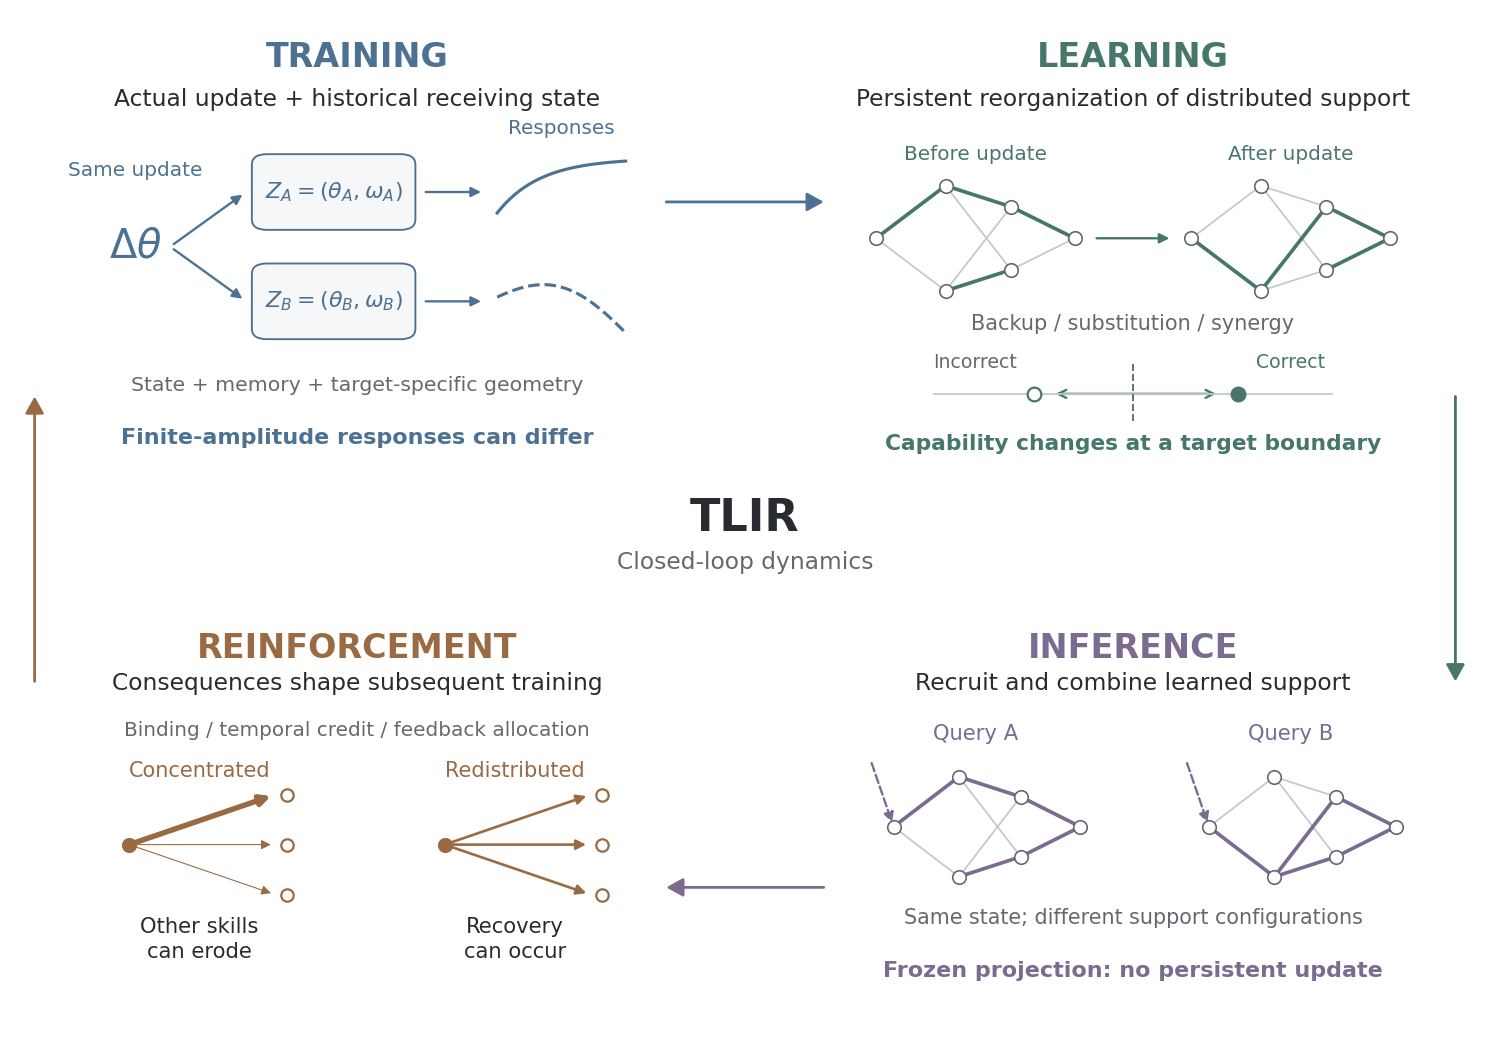
\includegraphics[width=.98\textwidth]{figures/figure1_tlir_closed_loop.png}
  \caption{TLIR closed-loop dynamics. Training, Learning, and Inference establish the open-loop core; Reinforcement feeds behavioral consequences into subsequent training.}
  \label{fig:chain}
\end{figure}
\begin{figure}[!htbp]
  \centering
  \captionsetup{font=small}
  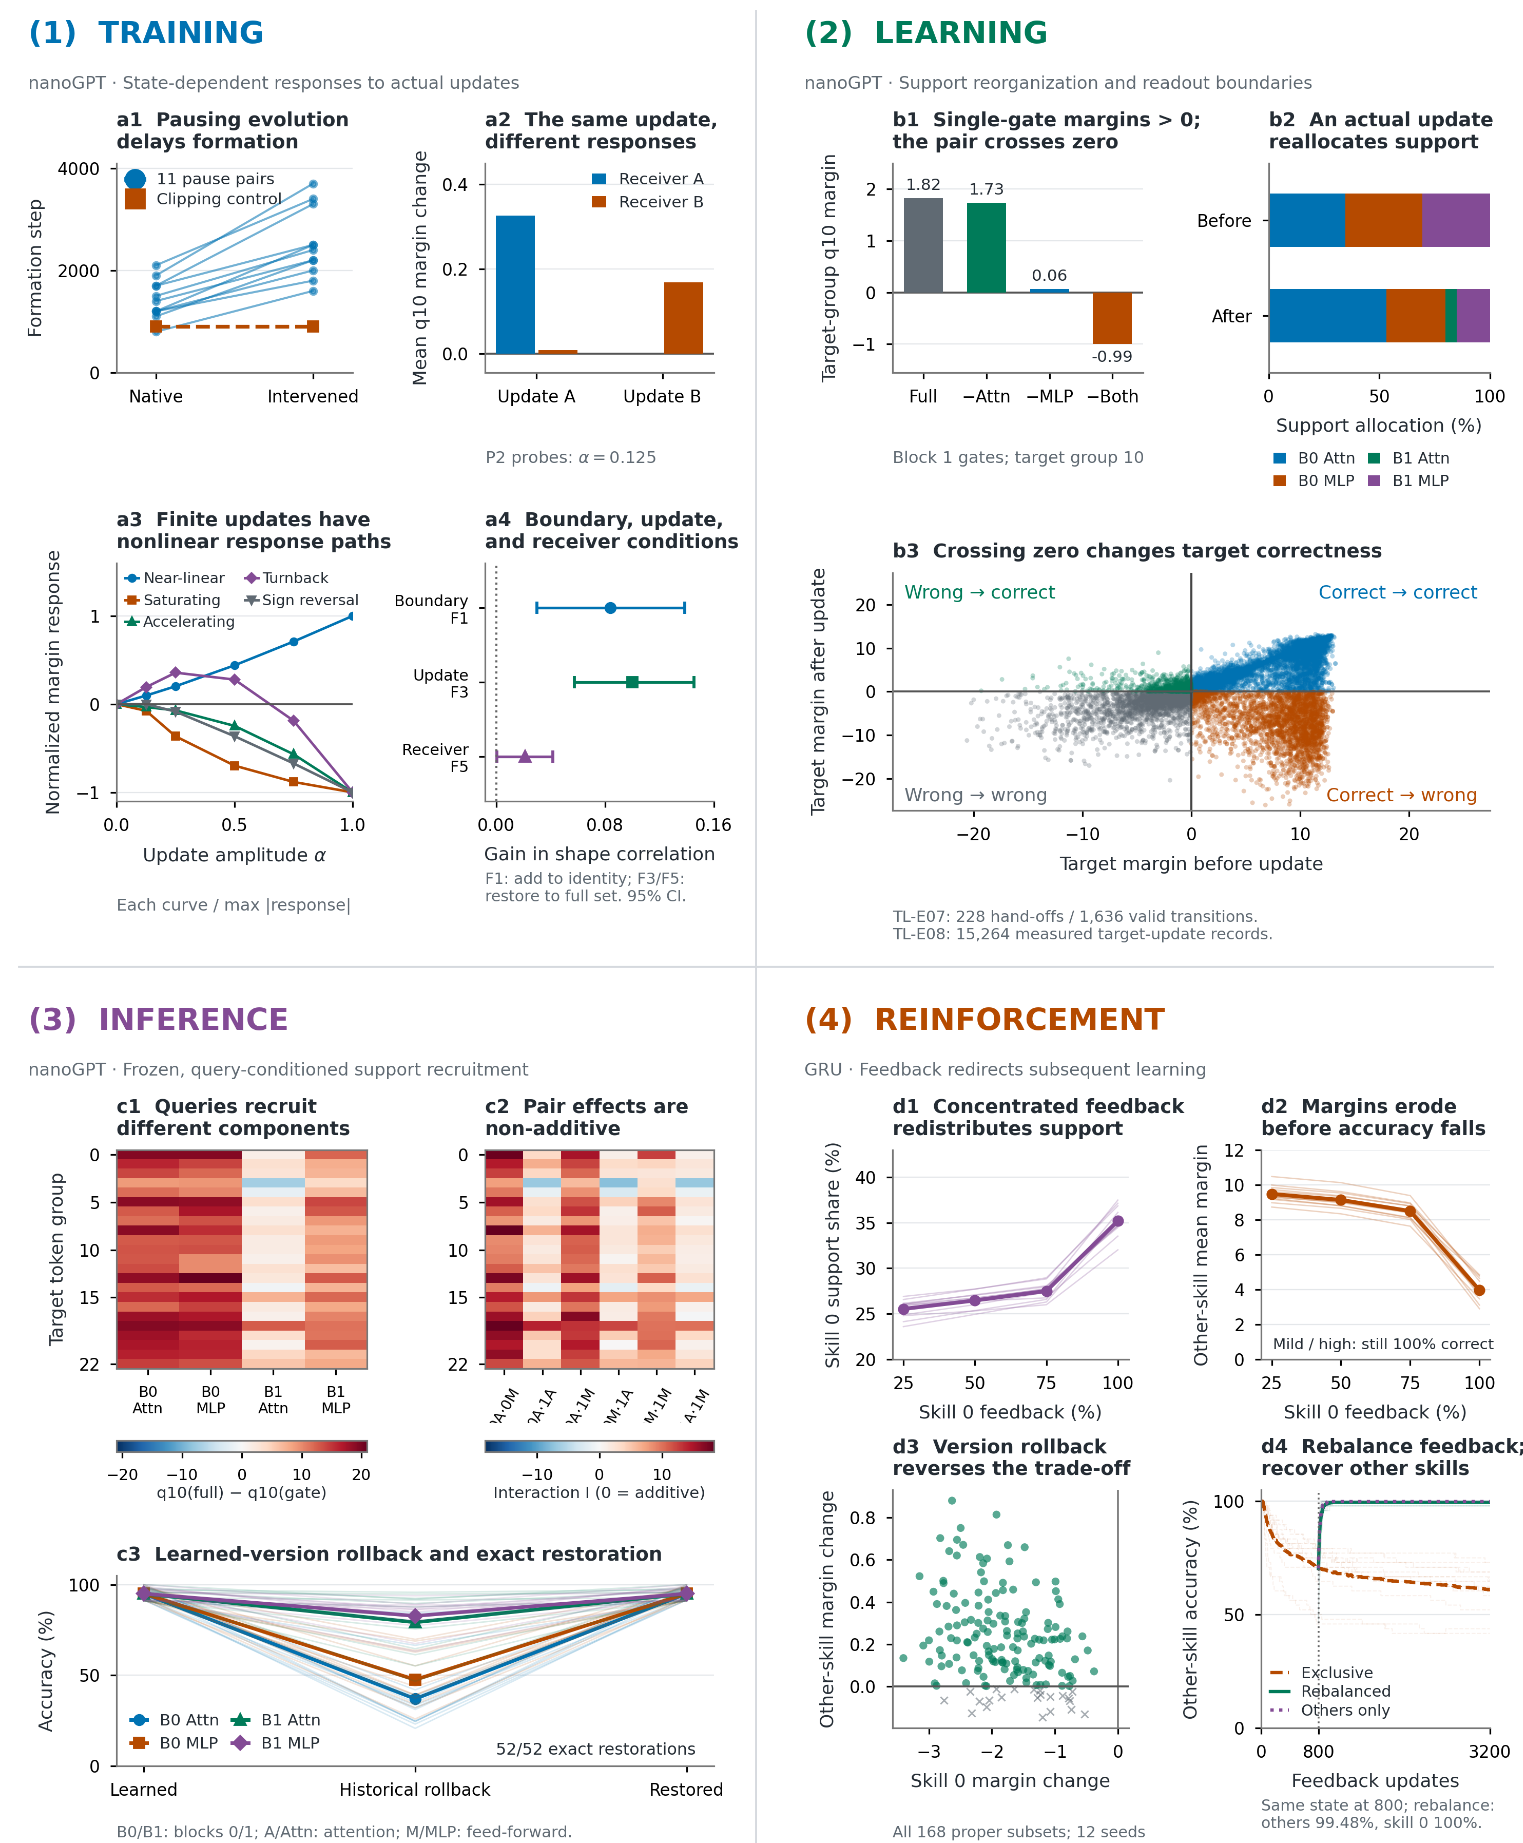
\includegraphics[width=1.00\textwidth,height=0.72\textheight,keepaspectratio]{figures/figure2_experimental_14panel.png}
  \caption{Selected evidence for Training, Learning, and frozen Inference in nanoGPT, and feedback-driven capability change and recovery in the shared GRU. (a1) Paused evolution delays capability formation; (a2) identical updates elicit different receiver responses; (a3) finite-amplitude response types; (a4) boundary, update, and receiver factors. (b1) Joint component removal crosses a target boundary; (b2) a realized update reallocates support; (b3) pre- and post-update target margins. (c1) Query-conditioned component effects; (c2) non-additive pair effects; (c3) learned-version rollback and exact restoration. (d1) Feedback-dose support redistribution; (d2) margin erosion before accuracy loss; (d3) rollback trade-offs; (d4) feedback rebalancing and recovery.}
  \label{fig:tlir-evidence}
\end{figure}
\begin{figure}[!htbp]
  \centering
  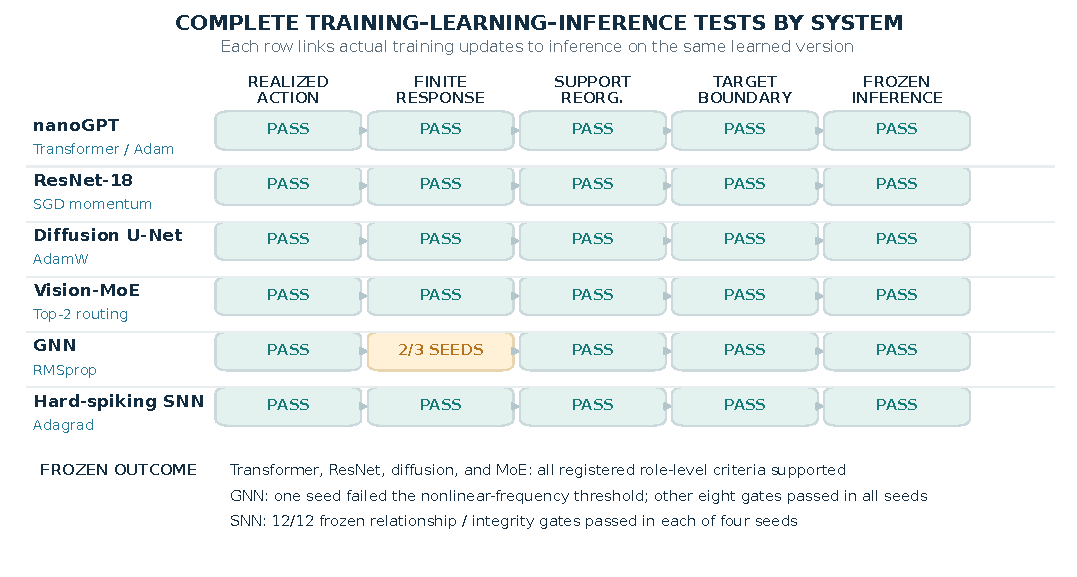
\includegraphics[width=.98\textwidth]{figures/figure2_six_system_evidence.pdf}
  \caption{Within-system training--learning--inference experiment chains. One GNN seed meets eight of nine registered gates, with nonlinear-response incidence below its specified threshold; SNN passes all twelve registered gates in four seeds.}
  \label{fig:systems}
\end{figure}
\begin{table}[!htbp]
\caption{Seven neural systems: six TLI chains and a GRU feedback study.}
\label{tab:systems}
\centering\small\setlength{\tabcolsep}{3pt}\renewcommand{\arraystretch}{1.07}
\begin{tabular}{@{}>{\raggedright\arraybackslash}p{.40\columnwidth}>{\raggedright\arraybackslash}p{.54\columnwidth}@{}}
\toprule
System (optimizer) & Task / registered components\\
\midrule
nanoGPT (Adam) & Cyclic next-token; 4 attention/MLP branches\\
ResNet-18 (SGD momentum) & CIFAR-100 classification; 4 residual stages\\
Diffusion U-Net (AdamW) & CIFAR-10 denoising; 4 U-Net paths\\
Vision-MoE (AdamW) & CIFAR-100 classification; 4 routed experts\\
GNN (RMSprop) & Graph reachability; 4 message-passing blocks\\
Spiking SNN (Adagrad) & 8$\times$8 digits; 4 spiking blocks\\
GRU (RL-E05/E06; AdamW) & Four-skill feedback; 4 shared hidden groups\\
\bottomrule
\end{tabular}

\end{table}
\begin{table}[!htbp]
\caption{Post-update target-boundary classification reports. Macro recall averages four observed transition categories; high accuracy alone is not sufficient. Predictor details and evaluation sets differ by system.}
\label{tab:prediction}
\centering
\setlength{\tabcolsep}{4.2pt}
\renewcommand{\arraystretch}{1.13}
\begin{tabular}{@{}lrr@{}}
\toprule
System & Accuracy (\%) & Four-way recall (\%)\\
\midrule
nanoGPT & 91.43 & 91.49\\
ResNet-18 & 99.28 & 97.99\\
Diffusion U-Net & 99.60 & 97.98\\
Vision-MoE & 99.63 & 96.95\\
GNN$^{a}$ & 98.54 & 98.62\\
Hard-spiking SNN$^{a}$ & 95.31 & 70.74\\
\bottomrule
\multicolumn{3}{@{}p{.94\columnwidth}@{}}{\footnotesize $^{a}$Independent prediction tests use registered GNN/SNN training histories.}\\
\end{tabular}

\end{table}
\begin{table}[!htbp]
\caption{RL-E06 feedback episodes per update, by capability.}
\label{tab:dose}
\centering\small\setlength{\tabcolsep}{4.1pt}\renewcommand{\arraystretch}{1.08}
\begin{tabular}{@{}lrrrr@{}}\toprule
Feedback & $q_0$ & $q_1$ & $q_2$ & $q_3$\\\midrule
Balanced & 15 & 15 & 15 & 15\\
Mild & 30 & 10 & 10 & 10\\
High & 45 & 5 & 5 & 5\\
Exclusive & 60 & 0 & 0 & 0\\\bottomrule
\end{tabular}
\end{table}
\newpage
\input{references.bbl}

\section*{Acknowledgments}
\paragraph*{Funding:}
This research received no funding.

\paragraph*{Author contributions:}
Mian Wang conceived the study; developed the atomic generation-fact model, the Generation-Fact Graph, the GFG-based recursive scientific process, and the unified theory of training, learning, inference, and reinforcement; defined the scientific questions, research boundaries, and decision criteria; introduced the principal theoretical hypotheses and conceptual transitions; directed the research program; analyzed and interpreted validated results; developed prospective predictions and theoretical deductions; prepared the figures; and wrote and revised the manuscript.

\paragraph*{Competing interests:}
There are no competing interests to declare.

\paragraph*{Data, code and materials availability:}
The study's public evidence repository is organized by the scientific claims of this paper to support rapid machine-assisted auditing (\url{https://github.com/wind342/tlir-research-evidence/tree/codex/tlir-paper-evidence-navigation-v1}). A paper-to-evidence map connects the main claims, experiments, figure panels, and reported results to frozen protocols, source code, result records, provenance and checksum manifests, and independent verification procedures. The public evidence matrix specifies which results can be independently recomputed and which underlying checkpoints or runtime artifacts are not included in the public release.

\paragraph*{Use of generative artificial intelligence:}
General-purpose AI systems, including OpenAI Codex and ChatGPT, served as scientific agents within the GFG-based recursive scientific process. Under the author's direction, these AI systems invented and implemented the four experimental instruments---CSRG-4C, realized-update causal forks, finite-amplitude update paths, and the identity-aligned target-boundary ledger---and designed, implemented, initiated, monitored, and executed the reported experiments. They performed analyses, causal interventions, matched replays, counterexample searches, and independent validation procedures, and contributed to manuscript drafting, editing, and LaTeX formatting. The reported numerical results were produced by the documented native programs and execution environments, not generated directly as text by AI models. The author defined the scientific questions, research boundaries, and decision criteria, reviewed the validated evidence, and accepts responsibility for the scientific claims and results.

\end{document}
